\documentclass[12pt]{article}
\usepackage{graphicx}
\usepackage[margin=30mm, paper = a4paper]{geometry}
\usepackage{minted, caption}
\usepackage{subcaption}
\usepackage{multicol}

\title{}
\author{}
\date{}
\setlength{\columnseprule}{1pt}
\setlength{\columnsep}{2cm}
\begin{document}
\vspace*{\fill}
\begin{center}

    \emph{Heaven's Light is Our Guide} \\
    \textbf{Rajshahi University of Engineering and Technology} \\

    \begin{figure}[h]
        \centering
        
\includegraphics[scale=.34]{images/RUET_logo.png}
        \label{fig:ruet_logo}
    \end{figure}
    \vspace{5mm}

    \textbf{Course Code}\\
    ECE 2216\\
    \vspace{3mm}
    \textbf{Course Title}\\
    Database Systems Sessional

    \vspace{5mm}
    \textbf{Experiment Date:} October 15, 2023,\\
    \textbf{Submission Date:} November 5, 2023\\

    \vspace{5mm}
    \textbf{Lab Report 3:} Creating a database and doing operations on it using SQL\\

    \vspace{15mm}

    \begin{tabular}{c|c}
        \textbf{Submitted to} & \textbf{Submitted by} \\
        Md. Robiul Islam      & Md. Tajim An Noor     \\
        Assistant Professor   & Roll: 2010025         \\
        Dept of ECE, Ruet     &                       \\
    \end{tabular}

\end{center}
\vspace*{\fill}

\pagebreak

\tableofcontents

\maketitle

\section{Tools Used}
\begin{itemize}
    \item MySQL
    \item VS Code - as an IDE to use SQL
    \item MacTeX -\LaTeX  compiler
    \item VS Code with LaTeX workshop extension as a text editor
\end{itemize}


\section{Process}


\subsection*{SQL Codes:}
\subsection{Previous lab's problems using join.}
\subsubsection{Find the customer name who are given highest commission.}
\subsubsection*{Code:}
\begin{minted}[breaklines, linenos]{mysql}
SELECT
    c.customer_name as "Customer Name",
    s.commission as Commission
FROM
    Relations.Customer c
    JOIN Relations.salesman s ON c.salesman_id = s.salesman_id
ORDER BY
    s.commission DESC
LIMIT
    1;
\end{minted}
\vspace{10mm}

\subsubsection{Find the amount of total commission given by salesman\_id = "5001".}
\subsubsection*{Code: }
\begin{minted}[breaklines, linenos]{mysql}
SELECT
    s.name as "Salesman Name",
    SUM(o.purchase_amount * s.commission) as "Total Commission"
FROM
    Relations.Order o
    JOIN Relations.salesman s ON o.salesman_id = s.salesman_id
WHERE
    o.salesman_id = 5001;
\end{minted}

\vspace{10mm}

\subsubsection{Find the salesman name whose customer’s grade is lowest.}
\subsubsection*{Code: }
\begin{minted}[breaklines, breakanywhere, linenos]{mysql}
SELECT
    s.name as "Salesman Name"
FROM
    Relations.salesman s
    JOIN Relations.Customer c ON s.salesman_id = c.salesman_id
WHERE
    c.grade = (
        SELECT
            MIN(grade)
        FROM
            Relations.Customer
    );
\end{minted}
\vspace{10mm}

\subsubsection{Find the total order number,ner from 5-9-2016 to 17-10-216 from the given table.}
\subsubsection*{Code: }
\begin{minted}[breaklines, breakanywhere, linenos]{mysql}
SELECT
    COUNT(o.order_no) as "Total Order"
FROM
    Relations.Order o
    JOIN Relations.Customer c ON o.customer_id = c.customer_id
WHERE
    o.order_date BETWEEN '2016-09-05'
    AND '2016-10-17';
\end{minted}
\vspace{10mm}

\subsection{New data.}

\subsubsection*{Creating the new tables and inserting data.}
\subsubsection*{Code:}
\vfill
\begin{multicols}{2}{|}
    \begin{minted}[linenos,breaklines,breakanywhere]{mysql}
CREATE DATABASE IF NOT EXISTS movie;

CREATE TABLE IF NOT EXISTS movie.movies(
    id INT AUTO_INCREMENT PRIMARY KEY,
    title VARCHAR(50),
    director VARCHAR(50),
    year INT,
    length_minutes INT
);

CREATE TABLE movie.box_office(
    movie_id INT,
    rating DECIMAL(3, 1),
    domestic_sales BIGINT,
    international_sales BIGINT,
    CONSTRAINT box2movies FOREIGN KEY (movie_id) REFERENCES movie.movies(id)
);

INSERT INTO
    movie.movies (title, director, year, length_minutes)
VALUES
    ('Toy Story', 'John Lasseter', 1995, 81),
    ('A Bugs Life', 'John Lasseter', 1998, 95),
    ('Toy Story 2', 'John Lasseter', 1999, 93),
    ('Monsters, Inc.', 'Pete Docter', 2001, 92),
    ('Finding Nemo', 'Andrew Stanton', 2003, 107),
    ('The Incredibles', 'Brad Bird', 2004, 116),
    ('Cars', 'John Lasseter', 2006, 117),
    ('Ratatouille', 'Brad Bird', 2007, 115),
    ('WALL-E', 'Andrew Stanton', 2008, 104),
    ('Up', 'Pete Docter', 2009, 101),
    ('Toy Story 3', 'Lee Unkrich', 2010, 103),
    ('Cars 2', 'John Lasseter', 2011, 120),
    ('Brave', 'Brenda Chapman', 2012, 102),
    ('Monsters University', 'Dan Scanlon', 2013, 110);

INSERT INTO
    movie.box_office (
        movie_id,
        rating,
        domestic_sales,
        international_sales
    )
VALUES
    (5, 8.2, 380843261, 555900000),
    (14, 7.4, 268492764, 475066843),
    (8, 8, 206445654, 417277164),
    (12, 6.4, 191452396, 368400000),
    (3, 7.9, 245852179, 239163000),
    (6, 8, 261441092, 370001000),
    (9, 8.5, 223808164, 297503696),
    (11, 8.4, 415004880, 648167031),
    (7, 8.3, 191796233, 170162503),
    (10, 8.3, 293004164, 438338580),
    (4, 8.1, 289916256, 272900000),
    (2, 7.2, 162798565, 200600000),
    (13, 7.2, 237283207, 301700000);
    \end{minted}
\end{multicols}

\vspace{10mm}

\subsubsection{Find the domestic \& international sales for each movie.}
\subsubsection*{Code:}

\begin{minted}[linenos,breaklines,breakanywhere]{mysql}
SELECT
    title as Title,
    FORMAT(domestic_sales, 'N') as "Domestic Sales",
    FORMAT(international_sales, 'N') as "International Sales"
FROM
    movie.movies m
    JOIN movie.box_office b ON b.movie_id = m.id;
\end{minted}

\vspace{5mm}
\subsubsection{Show the sales number for each movie that did better internationally rather than domestically.}
\subsubsection*{Code:}
\begin{minted}[linenos,breaklines,breakanywhere]{mysql}
SELECT
    title as Title,
    FORMAT(domestic_sales, 'N') as "Domestic Sales",
    FORMAT(international_sales, 'N') as "International Sales"
FROM
    movie.movies m
    JOIN movie.box_office b ON b.movie_id = m.id
WHERE
    international_sales > domestic_sales;
\end{minted}

\vspace{5mm}
\subsubsection{List all the movies by their ratings in descending order.}
\subsubsection*{Code:}

\begin{minted}[linenos,breaklines,breakanywhere]{mysql}
SELECT
    title as Title,
    rating as Rating
FROM
    movie.movies m
    JOIN movie.box_office b ON b.movie_id = m.id
ORDER BY
    rating DESC;
\end{minted}

\vspace{5mm}
\subsubsection{Find the movie ID, name of the movies that the highest length movie of each director.}
\subsubsection*{Code:}

\begin{minted}[linenos,breaklines,breakanywhere]{mysql}
SELECT
    m.id AS "Movie ID",
    m.title as Title,
    m.director as Director,
    m.length_minutes as "Length(Minutes)"
FROM
    movie.movies m
WHERE
    (m.director, m.length_minutes) IN (
        SELECT
            director,
            MAX(length_minutes) AS max_length
        FROM
            movie.movies
        GROUP BY
            director
    );
\end{minted}
\vspace{5mm}
\subsubsection{Find the local domestic sales of movies by John Lasseter so far.}
\subsubsection*{Code:}

\begin{minted}[linenos,breaklines,breakanywhere]{mysql}
SELECT
    director as Director,
    FORMAT(SUM(domestic_sales), 'N') as "Total Domestic Sales"
FROM
    movie.movies m
    JOIN movie.box_office b ON m.id = b.movie_id
WHERE
    director = 'John Lasseter';
\end{minted}

\section{Output}
\captionsetup{justification=centering}
\begin{figure}[htbp!]
    \begin{subfigure}{1\textwidth}
        \centering
        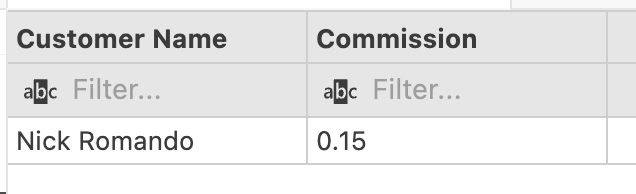
\includegraphics[width=\linewidth]{images/output/q1.png}
        \caption*{The person who is the top of the organization (i.e. reports to no one)}
        \label{fig:q1}
    \end{subfigure}
    \vspace*{20mm}
    \begin{subfigure}{.3\textwidth}
        \centering
        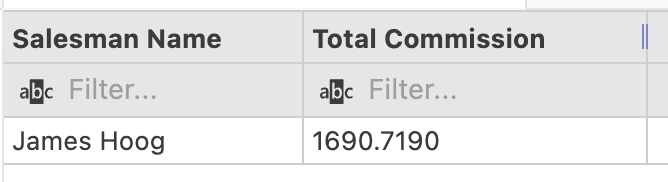
\includegraphics[width=.6\linewidth]{images/output/q2.png}
        \caption*{Difference in days between the most recent and oldest order date in Orders file.}
        \label{fig:q2}
    \end{subfigure}
    \begin{subfigure}{.3\textwidth}
        \centering
        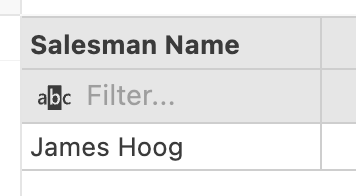
\includegraphics[width=.6\linewidth]{images/output/q3.png}
        \caption*{Total value of  payments received in July 2004.}
        \label{fig:q3}
    \end{subfigure}
    \begin{subfigure}{.3\textwidth}
        \centering
        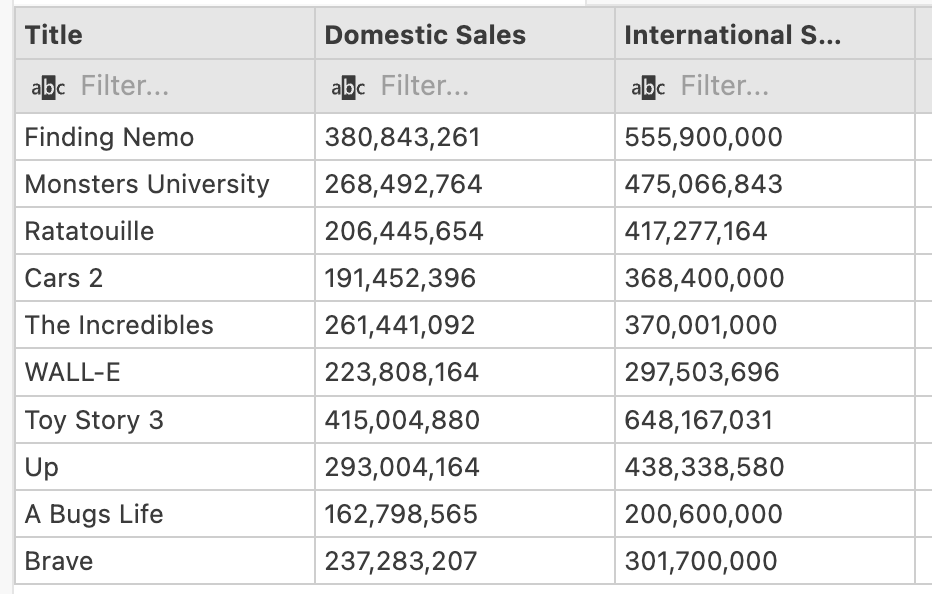
\includegraphics[width=.6\linewidth]{images/output/q6.png}
        \caption*{The number of orders ‘On Hold’ for each customer.}
        \label{fig:q6}
    \end{subfigure}

    \begin{subfigure}{\textwidth}
        \centering
        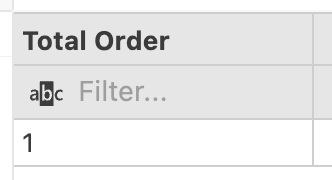
\includegraphics[width=.5\linewidth]{images/output/q4.png}
        \caption*{Profit generated by each sales representative based on the orders from the customers they serve. Sorted by profit generated descending.}
        \label{fig:q4}
    \end{subfigure}
    \begin{subfigure}{.5\textwidth}
        \centering
        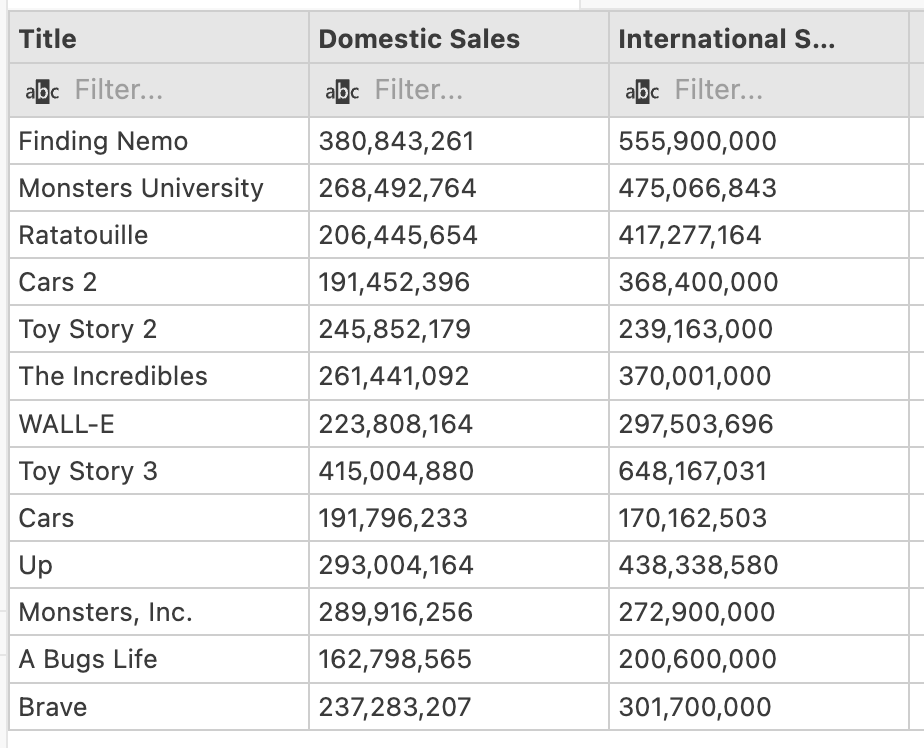
\includegraphics[width=.8\linewidth]{images/output/q5.png}
        \caption*{Products sold in 2003 but not 2004.}
        \label{fig:q5}
    \end{subfigure}
    \begin{subfigure}{.5\textwidth}
        \centering
        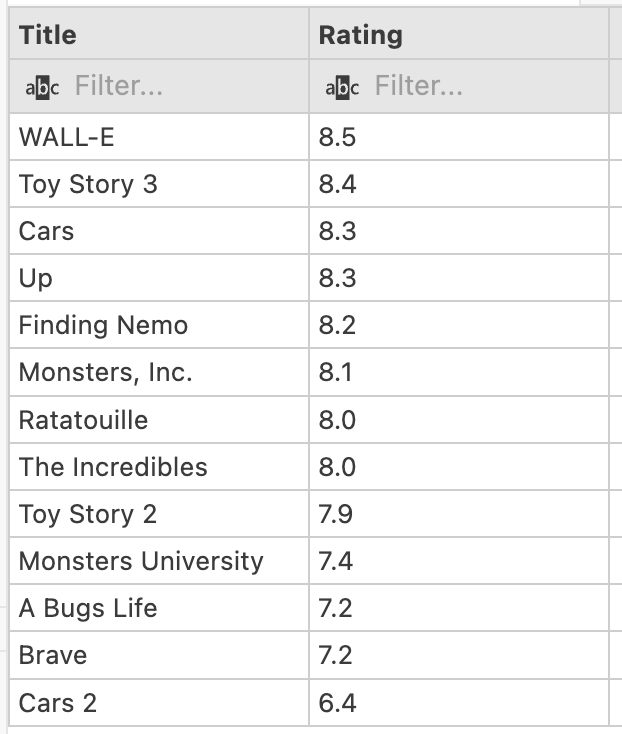
\includegraphics[width=.65\linewidth]{images/output/q7.png}
        \caption*{Names of products sold at less than 80\% of the MSRP.}
        \label{fig:q7}
    \end{subfigure}
\end{figure}

\pagebreak
\captionsetup{justification=centering}
\begin{figure}[H]
    \begin{subfigure}{1\textwidth}
        \centering
        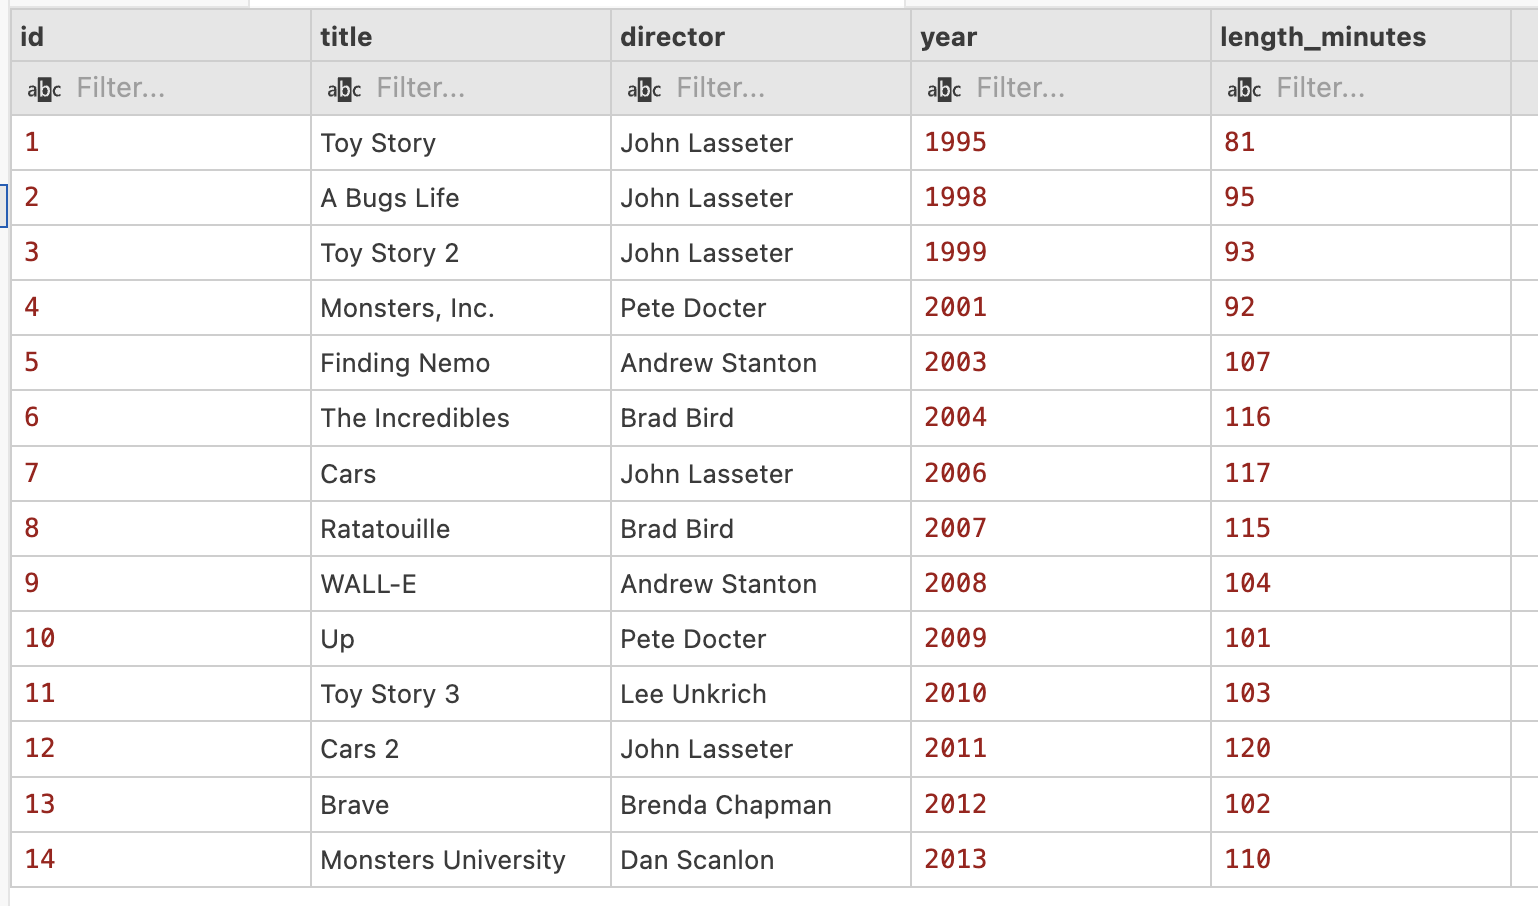
\includegraphics[width=.6\linewidth]{images/output/mov.png}
        \caption*{The complete Movies table.}
        \label{fig:mov}
    \end{subfigure}
    \begin{subfigure}{1\textwidth}
        \centering
        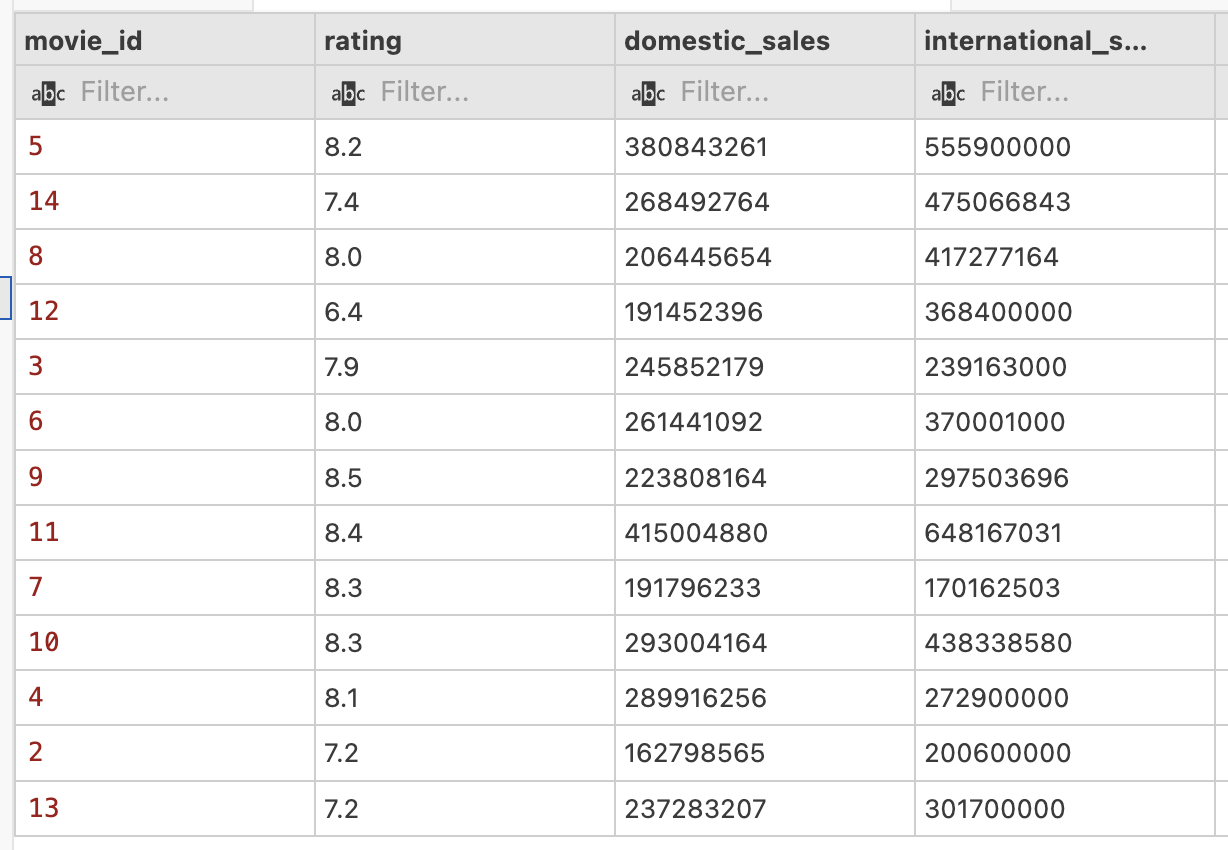
\includegraphics[width=.6\linewidth]{images/output/box.png}
        \caption*{The complete Box Office table.}
        \label{fig:box}
    \end{subfigure}
    \vspace*{10mm}
    \vspace*{10mm}
    \begin{subfigure}{.5\textwidth}
        \centering
        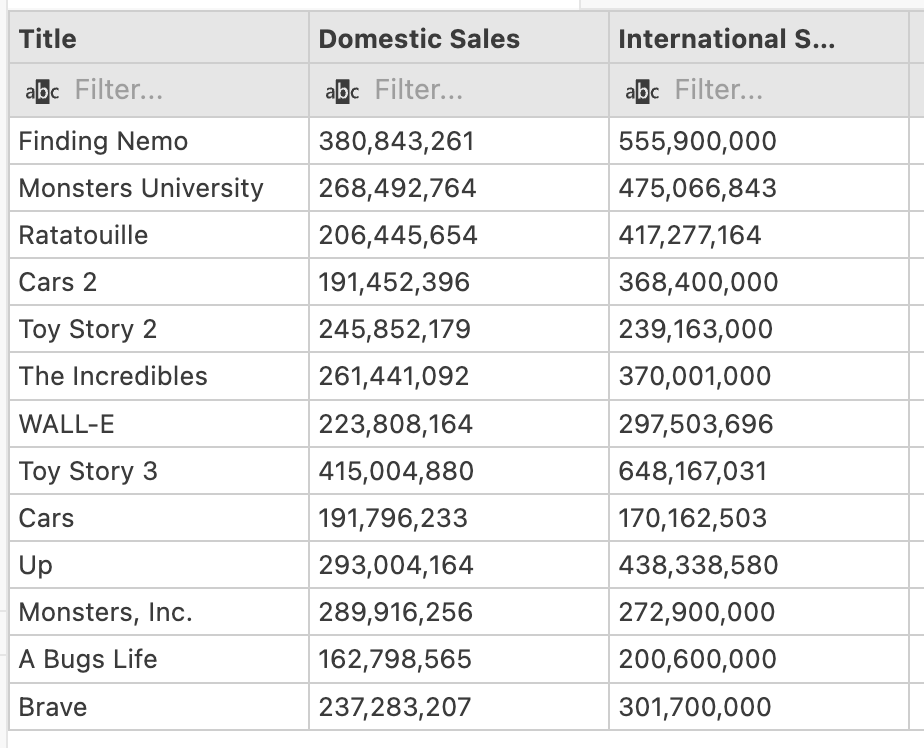
\includegraphics[width=.8\linewidth]{images/output/q5.png}
        \caption*{Domestic \& international sales for each movie.}
        \label{fig:q5}
    \end{subfigure}
    \begin{subfigure}{.5\textwidth}
        \centering
        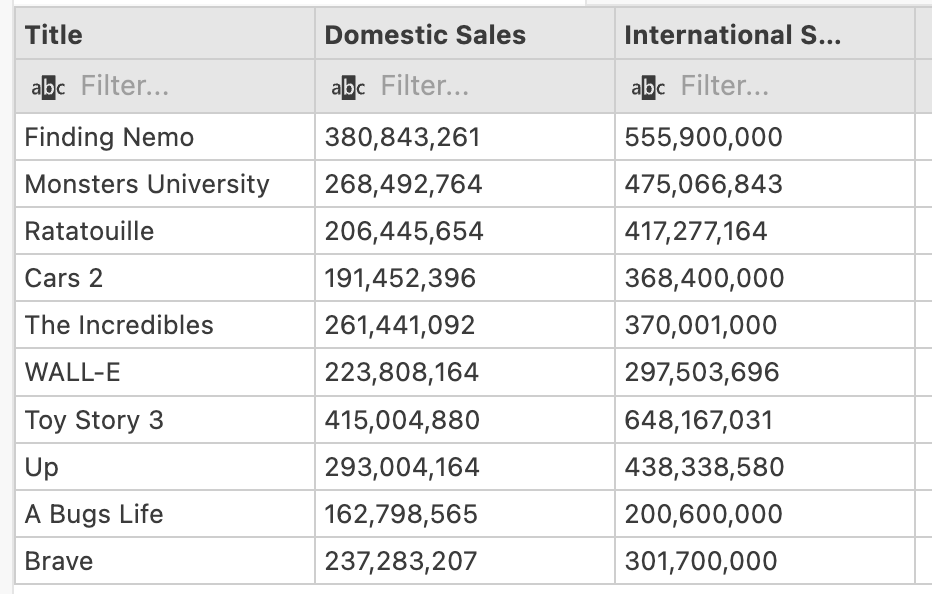
\includegraphics[width=.8\linewidth]{images/output/q6.png}
        \caption*{Sales for each movie that did better internationally rather than domestically.}
        \label{fig:q6}
    \end{subfigure}
\end{figure}
\pagebreak
\begin{figure}[H]
    \begin{subfigure}{.5\textwidth}
        \centering
        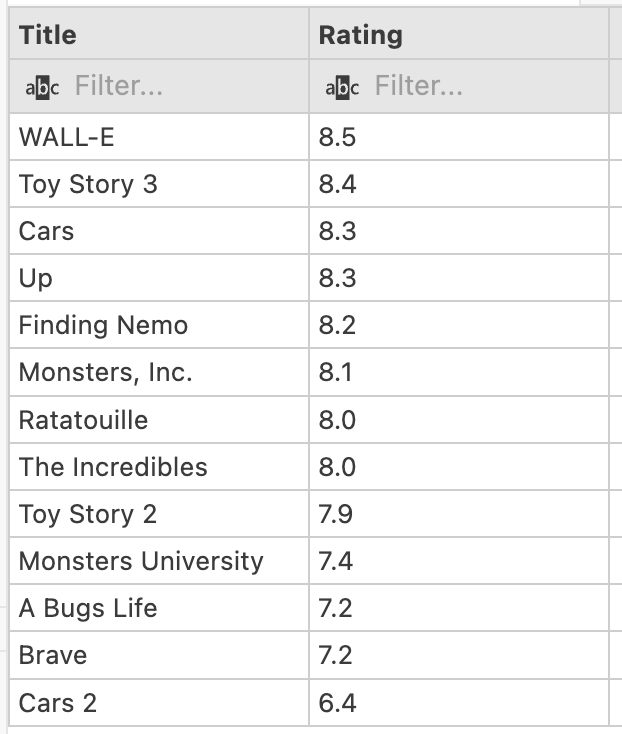
\includegraphics[width=.8\linewidth]{images/output/q7.png}
        \caption*{List of all the movies by their ratings in descending order.}
        \label{fig:q7}
    \end{subfigure}
    \begin{subfigure}{.5\textwidth}
        \centering
        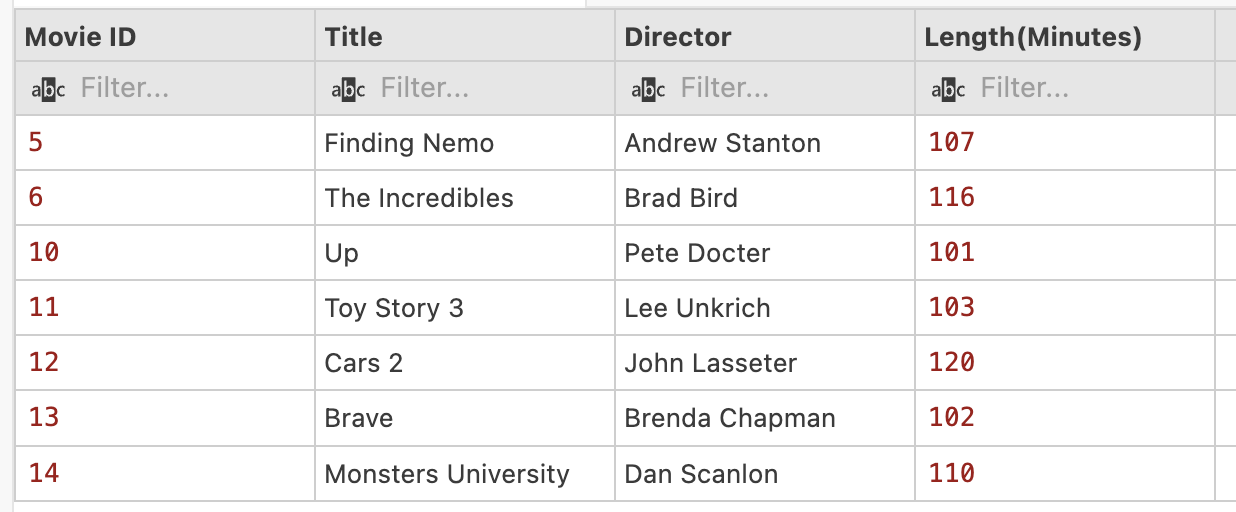
\includegraphics[width=.8\linewidth]{images/output/q8.png}
        \caption*{Movie ID, Name of the movies that the highest length movie of each director.}
        \label{fig:q8}
    \end{subfigure}
    \begin{subfigure}{\textwidth}
        \centering
        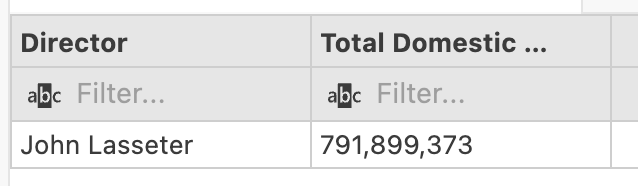
\includegraphics[width=.66\linewidth]{images/output/q9.png}
        \caption*{Local domestic sales of movies by John Lasseter so far.}
        \label{fig:q9}
    \end{subfigure}
\end{figure}


\end{document}